\fancyhead[LO]{{\scriptsize {\FA \ }我们最幸福 {\FA } 井底之蛙}}%奇數頁眉的左邊
\fancyhead[RO]{{\tiny{\textcolor{Gray}{\FA \ }}}\thepage}
\fancyhead[LE]{{\tiny{\textcolor{Gray}{\FA \ }}}\thepage}
\fancyhead[RE]{{\scriptsize {\FA \ }我们最幸福 {\FA } 井底之蛙}}%偶數頁眉的右邊
\fancyfoot[LE,RO]{}
\fancyfoot[LO,CE]{}
\fancyfoot[CO,RE]{}
\chapter*{13 {\FA } 井底之蛙}
\addcontentsline{toc}{chapter}{\hspace{5mm}13 \textbf{>}\ \ 井底之蛙}
\vspace{5mm}
\begin{flushright}
	\textcolor{PinYinColor}{\EN \huge{Frogs\\
	in the Well\\
	\ \\}}
\end{flushright}
\begin{figure}[!htbp]
	\centering
	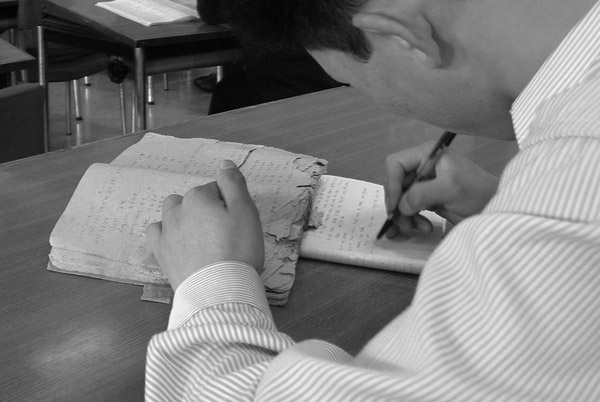
\includegraphics[width=6cm]{./Chapters/Images/13.jpg}
	\caption*{一名在北朝鲜最大的图书馆平壤人民大学习堂学习的学生}
\end{figure}


俊相在一次回家度暑假的时候,曾亲眼目睹过一次处决。执行前几天,带着扬声器的卡车就开着四处转,宣布着日期、时间。人民班班长也挨家挨户的敲门,通知每个人都被要求参加。俊相不喜欢这种场合。他恨血腥,他忍受不了看一个人或者动物受难。在他12岁那年,父亲强迫他去宰一只鸡。当俊相抓着鸡脖子的时候,手不停的抖着。“你连这个都不敢做,怎么成为一个男人啊?”父亲严厉的责备道。俊相只好顺从的用刀一挥,相对于一只无头的鸡,他更害怕父亲的斥责,但是当晚他拒绝吃晚饭。看着一个人死去对他来说是不可想象的事情。他发誓不会去看。但是当那天到来,所有的邻居都跑去看,他发现自己也跟不由自主的跟着人群一起走去。行刑地点设在离他和美兰夜晚散步去的那个温泉度假村不远的一条小溪的沙堤上。大概有300人已经聚集在哪里,孩子们推搡着想挤到前头。男孩们都想争抢公开处决时落下的子弹壳。俊相也挤过人群,想找个好的角度。\\

国家安全部门已经把场地整理了一下,变成一个临时的法庭,摆了些桌子用做检控席和摆放有两个巨大扬声器的扩音系统。那个人被指控爬电线杆盗剪铜线贩卖。\\

“这个窃贼导致了国家财产的巨大损失,意在破坏社会体系。这是叛国的行为,是帮助社会主义国家敌人的行为。”检察官朗读着,他的声音夹杂着扩音器的啸叫通过扩音器远远的传出去。然后有个人作为辩护律师对所做指控做出反应,然而他的话却没有丝毫辩护的意思:“我承认检察官所做指控均属实。”\\

“犯罪嫌疑人因此被判处死刑,立即执行。”第三人下令。\\

被宣告有罪的那个人的眼睛,胸口及腿就被绑在一个木桩上。行刑小组会按次序瞄准绑着的绳子,每个部位3枪,从上到下一共9枪。先是头部瘫软,然后身体按顺序瘫倒在脚下准备好的袋子里。简练且有效。看上去像是罪犯死了都在祈求原谅。\\

此时一股低声抱怨开始在人群中传出。看起来,不止俊相一个人认为对于这么小的一点偷窃就处以极刑实属太过于严厉。那些电线本来就没什么用。那个人偷的几米铜线可能换不了几袋米。\\

“真可怜,他有个妹妹。”俊相听见有人说。\\

“是两个。”另一个人说。\\

俊相猜想那个人的父母可能都死了。他肯定清楚没人会替他解决问题。他可能家庭成分也不好。可能像美兰的学生一样,是个矿工的孩子。\\

正当俊相思讨着这些可能性的时候,枪响了。\\

头、胸、腿。\\

头像个西瓜一样被打烂。鲜血立刻喷涌而出,几乎溅到人群的脚上俊相立刻觉得想吐。他马上扭头挤出人群,回了家。\\

对于俊相来说,每次去清津他总是会在自己的国家里有些令人不快的发现。在大学,俊相与最恶劣的现实相隔绝。他有足够的吃的,晚上也有电。平壤顶级大学的学生是这个特权城市里最具优先权的一群人。但是一旦离开了象牙塔,现实立刻面目狰狞的展现在眼前。\\

曾伴随美好记忆的地方现在都关门了。还是个孩子的时候曾去过的餐馆,第一次邂逅美兰的剧院。除了偶尔的公共假日,例如金日成和金正日的生日,其它时间都没有电。\\

夜晚都是摸黑在家,听着父母长吁短叹。他在东京富有的祖父已经去世,其它还活着的亲戚都不像祖父那么慷慨的给穷亲戚送钱。他母亲的风湿性关节炎也严重到让她无法步行去市场或者踩买自日本的缝纫机。\\

几乎每一个晚上都一样。父亲抽着闷烟,黑暗里烟头一亮一亮的。每吐一口烟,他就要重重的叹一口气,预示着他有坏消息要说。\\

“你知道谁死了吗?你还记得……”\\

他父亲提了俊相高中时一个老师的名字。他的数学老师。他的中文老师。还有他的文学老师,曾经也是个电影迷,还曾借给俊相几本电影文学的杂志给他看,那是关于东欧电影及电影在反帝国主义斗争中所扮演的角色等等。老师们大多是50多岁的知识分子,在学校系统停止发放工资后,他们发现自己没有什么其它的谋生技能。俊相过去在放假从平壤回家的时候,常常会去看望一下自己高中时期的老师们;老师们看到自己的学生如此优秀也是非常高兴。现在俊相会尽量避免联系高中的人。他不想听见谁又死了。\\

死亡不仅仅局限于老年人。俊相的母亲告诉他,他哪些同学饿死了,那些没有通过大学选拔考试不得不参军的人。俊相同他们都失去了联系,但是他曾经心安理得的想象他们应该能度过难关,因为士兵应该是优先供应食品的一类人。毕竟,是金正日自己宣称的先军(Songun)观点,或者“军事优先。”中小学生要做出牺牲,所以强大的军队就能保护他们免受美帝国主义的轰炸。\\

俊相现在可以看到那不是真的。清津附近的士兵们成群结队的,个个衣衫褴褛,用人造革腰带将不再适合他们骨瘦如柴身板的军服扎紧。因为营养不良,一个个的面露菜色,很多人身高仅及150公分\footnote{因为年轻一代生长状况不佳,北朝鲜军队在90年代早期也降低了新兵入伍所要求的160公分的身高标准}。一到夜里,他们一个个都擅离职守,爬进私人菜园,挖泡菜坛子,把蔬菜连根拔走。\\

住在附近的邻居们大多都加高了围着屋子的围墙,而无视于警方关于围墙不得高过150公分的规定,这样可以方便警察直接看到院内的情况。然而即使这样,窃贼还是光顾了三次,他们爬过围墙,将俊相家的菜园一扫而光。他们把种的大蒜,马铃薯和大白菜全部拔走。对菜园,俊相的父亲在他的蔬菜种植日志里做了很仔细的记录,记下他用的是什么类型的种子,以及发芽所需的时间。\\

“为什么他们就不能至少等这些菜长成啊?”他哀叹着。\\

当有人把狗偷走后,俊相的妈妈简直像失去了亲人。俊相还是个孩子的时候,她就养了这只丰山犬。她非常溺爱这只狗,每天亲自给它做吃的。在写给在大学读书的儿子的信中,也满是这只小狗的消息。她容忍不了这只狗很有可能已经被吃掉了的想法。\\

实际上,他们非常的幸运,只是狗被杀了而已。每个人都知道他们家来自日本,有钱,所以他们很容易被窃贼盯上。他们村子里有一户人家在一次令人发指的抢劫中,全家被杀。俊相和他家必须比以前更加小心。他们在高墙后的房间里快速吃完晚餐,希望不要被邻居看见他们有足够的吃的。\\

自从对金日成的死无法挤出眼泪以来,俊相意识到他对这个体系的失望是与日俱增。任何他所看到,所听到的,所读到的,都使得他与所谓的政治正确的思考渐行渐远。他在大学的经历改变了他。生命里第一次他有了全新的观点。\\

当还是个孩子的时候,俊相读所有他能弄到的书。小说、哲学、科学、历史甚至是金日成的演说。镇子上的书店卖的小说讲述着美国佬的凶残,南韩人的谄媚、懦弱,以及英雄的北朝鲜人。偶尔也会有俄罗斯的小说,托尔斯泰(Leo Nikolayevich Tolstoy)或者高尔基(Maxim Gorky)的著作。他高中时期所看的书都是来自教育器材及读物供应办公室以及他父亲那颇为可观的关于希腊和罗马历史的藏书。俊相很爱读那些古代勇士的书。他喜欢关于汉尼拔(Hannibal)是如何将罗马帝国搅得天翻地覆,宁可服毒自尽也不愿接受失败的那些故事。\\

等他到了平壤,他已经做好准备迎接更现代的事物。在大学里,图书管理员的桌子后面,有一小部分经过挑选的翻译成朝鲜语的西方书籍。这些书是不准面向普通大众的;只有顶级的学生可以接触这些书。在政府的某个高级层面,有人决定这个国家也需要一些精英学生对西方文学的精华有所瞭解。这些书在封面上没有标明出版社名称,但是俊相听见有传言说它们是由人民大学习堂(Inmin Daehakseupdang)\footnote{人民大学习堂是一个位于金日成广场,橱窗式的国家图书馆。}出版。这些书里甚至还有美国的书。\\

俊相最爱读的是《飘》(Gone with the Wind)。这种通俗风格的书不同与朝鲜小说的语调。他惊讶于美国内战和朝鲜战争是何其相似。他很惊奇的发现同一人民之间的战争竟会是如此激烈、血腥──很明显美国人同朝鲜人一样慷慨激昂。他想美国人的结局更好,毕竟美国最终还是归为一统,而不像朝鲜人至今仍然分裂着。他很钦佩于女英雄郝·思嘉(Scarlett O{\EN '} Hara),钦佩她的勇敢。她也小小的提醒了他,在北朝鲜电影里也有个女英雄,总是在泥地里摸爬滚打,为祖国而战,但是郝·思嘉(Scarlett O{\EN '} Hara)更多的是个人主义者。这在北朝鲜文学中是不值得赞扬的。而且北朝鲜的女英雄肯定是没有卿卿我我的爱情。\\

按照北朝鲜的标准这些可是伤风败俗的。俊相还想读更多的书。他读完了所能找到的所有的书,从西德尼·谢尔顿(Sidney Sheldon)的《天使的愤怒》(Rage of Angels)到加西亚·马尔克斯(Gabriel Garcia Marquez)的《百年孤独》(100 Years of Solitude)。他甚至还读了《人性的弱点》(How to win friends and influence people),卡耐基(Dale Carnegie)写于30年代的自立励志经典。这是他第一次对西方商业的探索,而且这深深震动了他。他不能相信卡耐基给读着的种种建议。\\

学会爱、尊重并以愉快与人相处。\\

一个在美国的资本主义体系下的作品怎么会像这样写?俊相问自己。难道所有的资本主义敌人不是生活在丛林法则中吗?要么杀人、要么被杀。\\

俊相还从同学那里借书。在顶级的大学,很多学生有一些位高权重的亲戚,他们时常出国,能买些书籍杂志。朝鲜语的材料在中国延边地区可以买到,那里有很多朝鲜族人口。通过他的一个同学,俊相还得到一本中国学校系统出版的性教育读本。真是大开眼界!俊相意识到他和他那些20多岁未婚朋友的性知识还不如中国的中小学生。为什么他要知道女性的生理周期?那能解释很多东西。\\

他还吃惊的读到一个在共产党代表大会上印发的讲话,讲话批判了毛发动的文化大革命。总有一天,他想,劳动党也会批判金日成。\\

一天,一个和俊相经常交换书籍的同学偷偷靠近他。这个学生四下看看,然后很神秘兮兮的塞给他一本书。\\

“这本书很好。”他耳语到。“可能你想看看?”\\

书是一本薄薄的俄罗斯政府出版的关于经济改革的小册子。那个男孩的爸爸在平壤一个书展上,在俄罗斯大使馆那里得到的。书看上去是90年代初,当俄罗斯试图建立自由市场经济改革时写的。俊相立刻意识到这本书在手上的危险,北朝鲜人被要求将任何他们发现的外国文学上交给警方。他、男孩、还有男孩的父亲都会因为私藏这样的书而惹上大麻烦。俊相马上把书藏到自己更衣箱的衣服下面。他的宿舍有两张上下床,四个学生一间,所以他们很少有私人空间。他只能躲在被子里用手电筒偷偷的看。\\

他读到:在早期阶段,资本主义是一种无情的竞争,目的是追求财富。此时没有公平分配社会财富的概念,或者普通工人福利的概念。经济以一种无序的方式发展……但是现代资本主义已经有非常大的进化,已经纠正了之前的缺点。例如,反托拉斯法\footnote{反垄断法。}确保正常有序的生产,但是生产活动不由国家控制。\\

这本书继续解释退休金制度和保险、福利的概念。它阐述了全球范围内社会主义经济体系的崩溃是缘于他们的无效率。俊相发现他边读边不由自主的点着头。\\

在1996年,俊相拿到了大学文凭。没有回清津,他决定继续留在学校,读研究生。他现在正式是个成年人了,有权搬出校园。他搬出了学校宿舍,租了间私房。这是一间破旧,肮脏的房间,没什么家具,但是他很喜欢他的房东,一对老年夫妻,耳朵有点背,眼神也不好。他们完全符合俊相的预想。一旦有个自己的房间,俊相用祖父最后一次来给的钱买了台索尼电视机。然后按北朝鲜法律,他在无线电监察局对电视机进行了登记。由于北朝鲜自己不能自行生产家用电器,进口的电视机必须将频道固定至官方电视台,然后将调频器失效,安装北朝鲜版本的去功能软件,这样就防止电视被用于接收外部世界的信号。北朝鲜人自嘲他们就像个“井底之蛙。”世界对他们来说不会比头顶上的那一片天空大。技术娴熟的人很快就能搞定,避开这个系统。对于收音机来说,这很容易。只要打开后盖,切断联系表盘的传送带,再换上橡胶圈,这样就可以转到你想要的任何频道。电视就要多一些的专业技术。\\

这个局会贴个纸封条在电视机的按钮处,这样证明电视机业已预设好,处于批准状态。要绕开封条又不损坏它,俊相用一根又长又细的缝衣针去按按钮。在他房间里有个后门通往外面的院子,在那他安了一部天线。在所有人睡了之后,他调试天线,通过调整不同天线的方位,最后找到了他想看的:南韩电视节目。\\

俊相只有当夜深了,来自非军事区以南150公里的电视信号最清楚的时候才开始听电视节目。他会一直等到自己确信房东都已入睡。因为墙壁非常薄,他能听见他们打呼噜。由于电视没有设置耳机插孔,他不得不把电视的音量调到刚刚能听到的程度。而他要屈膝,把耳朵贴到扬声器上,直到他的腿和脖子酸的坚持不住这个姿势了。与其说他看电视,不如说他是在听电视。当打开电视的时候,他总是处于高度警惕的状态。几个门之外,有个邻居养有一条狗。如果他夜里听见狗叫,俊相就会马上把电视调到官方电台,并且飞奔出去把天线藏起来。\\

电视核查人员确实会来。有一个眼睛非常毒,他注意到一片透明胶带纸贴在纸封条上。俊相用胶带纸掩盖针在纸上留得痕迹。\\

“这个胶带纸是干什么用的?”核查人员问道。\\

俊相的心狂跳。他曾听说有一户人,家里有人看了南韩电视节目,而全家都被送往古拉格(劳动营)。他的一个朋友仅仅是被怀疑听了南韩的广播就被审讯了整整1年,而在此期间他从没有见过阳光。当他被释放的时候,他脸色像死人一样的苍白,他精神几乎崩溃。“哦,我贴上胶带纸怕它松开。”他故作镇定的回答道。核查人员皱了皱眉,走开了。\\

在这次侥幸逃脱之后,俊相更加小心了,但是他实在不能抑制自己的好奇心。他现在对信息,特别是实时信息的胃口变得越来越大了。电视带给俊相的不仅仅是外面世界的新闻,更多的是,他以前从不知晓的自己国家的信息。\\

俊相了解到很多令人瞠目结舌的事情,那些他曾经怀疑过但却从不知晓的。他听到比尔柯灵顿总统说美国已经提供燃油和能源援助,但是北朝鲜却没有停止研发核武器和导弹。他发现美国提供给北朝鲜以几十万吨的大米作为人道主义援助。\\

数名美国国会成员组成的代表团举行了个新闻发布会宣传北朝鲜的饥荒导致多达200万人死亡。人权组织估计20万人被关押在古拉格式的劳动营里,北朝鲜有着全世界最差的人权纪录。\\

在2000年,南韩的电视台报导南韩总统金大中即将在平壤同金正日进行历史性的峰会。峰会期间,南韩电视台播放了金正日的声音,当时他同南韩总统在谈话。俊相以前从没有听过敬爱领袖的声音;在北朝鲜广播和电视中他的讲话,都是由一个专业的播音员,以一种颤抖的、充满敬畏的嗓音朗读出来。这样可以保持他的神秘感。“你怎样看我们的历史名胜?”俊相听见敬爱的领袖以一种听上去很苍老、无力但是却很清楚的声音说。\\

“毕竟他也只是个人,“俊相这样对自己说。\\

听南韩的电视节目就像是一个人一辈子第一次照镜子,意识到自己并不是那么可人。北朝鲜人总是被告知他们是世界上最值得骄傲的国家,但是外面的世界却认为它是个可怜的、破产的政权。俊相知道人们在挨饿;他知道人们被强制投入劳动营;但是他从来不知道有多少。当然,南韩的新闻报导可能夸大其词,但是,会像北朝鲜宣传部门那样不靠谱吗?\\

俊相回家的火车之旅,让他不禁想到自己读的佛教经文中所描述的人间地狱。车厢里是如此拥挤以至于他无法去上厕所。男人就直接往车窗外尿,要不就等到停车的时候,到野外去尿,但是有时候他们连着都无法做到,只好在车厢里解决问题。当车慢些的时候,无家可归的孩子就会在车箱旁追着跑,乞讨,有时候还会尖声乞求食物。他们还会试图从破车窗外伸手进来抓吃的。火车总是严重晚点,因为在试图爬过平壤以北陡峭的山坡时,车头经常会趴窝。俊相有一次被困于发生故障的火车里长达两天,那时正处严冬,寒风肆虐着没有窗户的车厢。他也尽可能的帮助同其它乘客。一个妇女带着一个20天的婴儿,还有一个因晚点而缺席了自己婚礼的年轻人。他们在一起,弄了个金属桶,在里面生起了火,而不理会列车员要求把它拿出去的命令。如果不是这堆火,他们可能全部都因体温过低而见了阎王。\\

在北朝鲜经济跌至谷底的1998年的一次旅途中,俊相被困于咸镜南道的一个小镇,通常他在那里转车,从向东的车转到沿着海岸向北的车。铁道被洪水淹了,暴雨把等车的乘客浇了个透心凉。俊相在站台上找一切可以避雨的地方。当等着的时候,他注意到有一群无家可归的孩子,流浪的燕子(Kochebi),在卖艺讨钱买吃的。有些孩子耍些小魔术,有些跳舞。有一个男孩,大概7-8岁,在唱歌。他细小的身体藏在成人尺寸的工装里,但是他的发音听上去又远比年纪大。他紧闭着双眼,满怀深情的唱着歌,整个站台都被他的歌声感染着。\\

\begin{quote}
	\begin{spacing}{1.0}  %行間距倍率
		\textit{{\footnotesize 	Uri Abogi,我们的父亲,这个世界上我们无所羡慕。\\
		我们的家园在劳动党的怀抱之中。我们都是兄弟姐妹。\\
		即使面对火海,可爱的小朋友们请不要害怕。\\
		因为父亲在这里。\\
		这个世界,我们无所羡慕。\\}}
	\end{spacing}
\end{quote}

俊相很小的时候就牢记此歌,除了现在的歌词有点更改。在这句个词中“我们的父亲,金日成。”这个孩子将名字换成了金正日。即使真的,这么小的孩子也不应该为能给予他保护的父亲唱赞歌,况且他的境况也很明显的与歌中所唱的不符。现在他在站台上,全身湿透、污浊不堪而且毫无疑问的饿着肚子。\\

俊相摸了摸口袋,给了这个孩子10元钱,对街头艺人来说这是一个慷慨的小费了。虽然有部分怜悯,但是更多的感激这个孩子带给他的反省。\\

后来,他想他应该感谢这个孩子使他清醒过来。现在他明白了,自己完全不信那一套。这是真情流露的重要时刻,正如一个人决定放弃信仰成为无神论者一样。这让他感度无比孤独。从此他将与他人格格不入。就这样,他突然无意识的就背负上自己发现的关于自己的一个秘密。\\

心里的疑惑澄清了,起先他以为他的生活将会因此有翻天覆地的变化。事实上,生活和以前一样没有一丝涟漪。他又仔细思考了一次自己所忠于的观点。在周六的早晨,他会准时的出现在大学的意识形态讲座中。劳动党党委书记喃喃的述说着金日成的传奇,听上去他好似一部自动播放机。在冬天,当礼堂的暖气还没有开启的时候,演讲者就会以最快的速度敷衍了事。俊相会经常偷偷的观察其它的听众。参与讲座的通常会有500人左右,大多是研究生或博士后。整个讲座期间,他们一个个都晃着脚,把手放在屁股下取暖。但是他们的脸很平静、木无表情、麻木的如同百货商店橱窗里的人体模型。\\

他突然意识到他的脸上也挂着同样的表情。实际上,对于讲座的内容,他们可能和他有着一样的看法。\\

“他们知道!他们全都知道!”他几乎要喊出来了,他非常确定。他们应该是这个国家最为聪明的头脑。“任何有脑子的人不可能不知道,这不对头。”\\

俊相意识到他不是唯一不信的人。他甚至认为他能以一种保持沉默的交流方式认出这些同类,这种方式很微妙,甚至没有到眨眼,点头的程度。他们大学里有个学生,年轻女性,在日记里叙述着她是如何的爱戴着亲爱的领袖,赢得不少赞扬。《劳动新闻》还有关于她的报导,她也因为自己的忠诚而受到褒奖。大学的学生们却刻薄的挖苦她。他们认为她是个怪人,但是因为他们不可以这样说,于是就嘲讽她。\\

“谁那么幸运能娶到你啊?”他们问她。但是他们能做的也就仅此而已。\\

北朝鲜的学生和知识分子同其它共产党国家的同行一样不敢上街示威。在北朝鲜没有布拉格之春,没有天安门广场事件。北朝鲜的高压程度是如此之高,以至于没有任何有组织反抗的苗头。任何参与反政府行为的示威者,他的直系亲属,以及所有知晓的亲属,都将得到可怕的惩罚。在这样一个三代以内连坐的体系下,惩罚将延伸至父母、兄弟、姐妹、侄子、侄女、表亲。“很多人觉得如果用他们的生命换取终结这个可怕的政权,他们愿意这么做,但是问题是你不是唯一受惩罚的人。你的整个家庭全部都要被打入地狱。”一个脱北者这样告诉我。\\

在北朝鲜,想成立读书俱乐部或者进行一个政治研讨是不可能的事情。任何自由的交换思想观点都将不可避免的延伸至禁区。在任何3或4人的小团体中,就至少会有一个告密者或者各种各样的特工。俊相怀疑他高中里一个最好的朋友就是政府的线人。这个男孩曾是学校最好的学生,甚至比俊相还优秀,但是他上不了平壤的大学,因为幼年时曾患小儿麻痹,导致腿跛。当俊相从平壤回家的时候,这个朋友就会大声的抱怨政府,且鼓励俊相应答。他的话语大胆而又有点做作,这使得俊相很担心这是个陷阱。后来俊相对他就完全避而不见了。\\

他提醒自己:只要你还住在北朝鲜,你就不可谈论政治。对你最好的朋友不能,对老师甚至是父母不能,当然对你的女友也不能。俊相从来不在美兰面前谈及对这个政权的感觉。他没有告诉她,他在看南韩电视,读资本主义小册子的事情。他当然也没有告诉她,他已经开始幻想叛逃。\\
